\subsection{Resolving the ethylene extension with a common screened reference}
The prospective ethylene discrepancy motivates a second, separately
identified development candidate. The F reference represents the full DFT
Fock operator in a confined valence image, whereas its qualified Q levels
come from the larger DFT calculation. To assess this imbalance, let $P$
be the isometric native-valence image and $Q$ its orthogonal complement
in the complete DFT orbital space. For an already qualified orbital match,
we evaluate the diagonal complement self-energy
\begin{equation}
 \Sigma_i(E_i)=F_{iQ}(E_i-F_{QQ})^{-1}F_{Qi}
\end{equation}
at its matched DFT orbital energy and add it to the F level before the
unchanged 50/50 average. Unqualified matches retain their original reference.
This is a diagonal downfolding approximation, not an exact many-electron
elimination of the DFT environment. No excitation reference enters this
one-body preparation. It lowers the ethylene result from 9.079 to 8.206 eV,
consistent with a substantial confinement contribution to the initial error.

The environment screening is rebuilt using Coulomb vertices between native
occupied orbitals and an explicit orthogonal DFT bath, avoiding the use of
missing active-orbital spectral weight as an independent screening channel.
Subspace disentanglement is a recognized issue in constrained
screening.\cite{miyake2009} We allow one global semiempirical efficiency
$\eta$ for this additional bath polarization:
\begin{equation}
 W=L_P^\mathrm{T}
 \left[I+B_NB_N^\mathrm{T}+\eta B_BB_B^\mathrm{T}\right]^{-1}L_P .
\end{equation}
Here $B_N$ contains the retained native environment transitions, $B_B$
the occupied--bath transitions, and $L_P$ the native Coulomb vertices.
The one-body interaction is normal ordered to the corrected native ground
Fock. The retained configuration space is unchanged. Static screening is
an approximation whose quantitative limitations also arise in molecular
RPA downfolding.\cite{verzijl2026}

We calibrate $\eta=0.60$ by balancing the opposite errors of furan V010
and furofuran C002, and freeze it before evaluating the complete ledger.
This is \emph{one fitted interaction parameter}; it is neither an energy
offset nor a parameter-free correction. It applies to every molecule and
state. The F/Q weights stay 50/50, exchange-response $\lambda$ stays 0.9,
and orbital gaps are not multiplied by either parameter. All 23 numerical
labels have been exposed during development, including the three-state
extension, so this assessment is not a blind validation.

\begin{figure}[!htbp]
\centering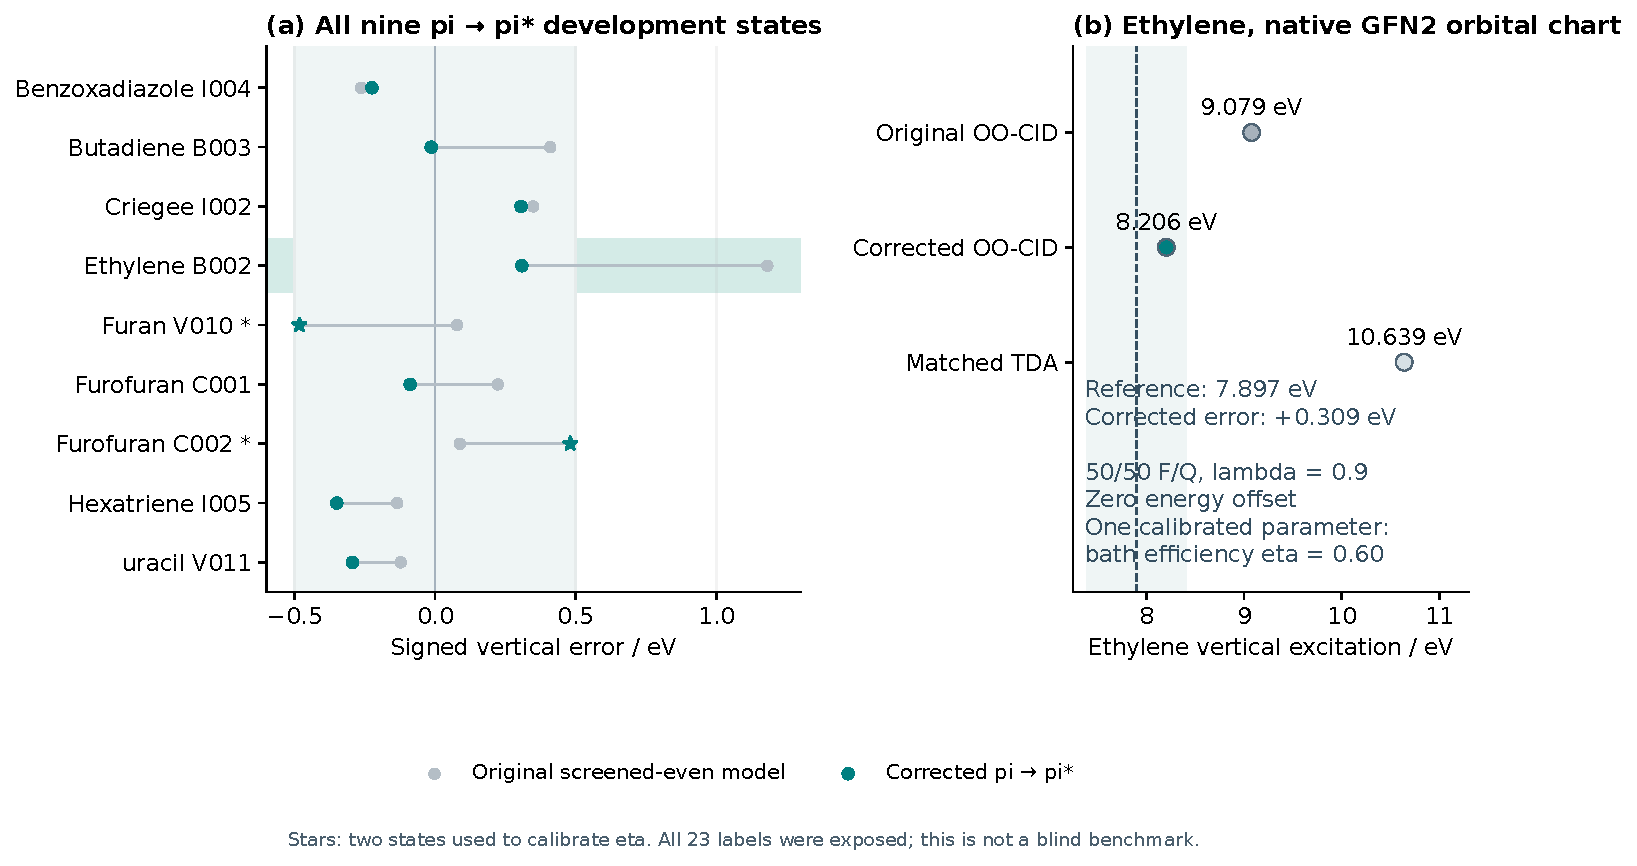
\includegraphics[width=\linewidth]{figures/ethylene_repair.pdf}
\caption{Common-reference repair on the complete exposed development set.
(a) Original and corrected signed errors for all nine $\pi\pi^*$ states; stars identify
the two states used to calibrate bath efficiency $\eta$. (b) Ethylene's
initial and corrected OO-CID energies, with a freshly evaluated TDA control
using the corrected native GFN2 ground orbitals and reference response.
The reference is 7.897 eV. The shaded intervals are $\pm0.5$ eV.}
\label{fig:ethylenerepair}
\end{figure}

All nine $\pi\pi^*$ states now lie within 0.5 eV, with MAE 0.283 eV and
maximum error 0.482 eV. The fourteen $n\pi^*$ states give 0.175 eV MAE
and 0.381 eV maximum error. All 23 states give 0.217 eV MAE. The 21 states
not used to choose $\eta$ give 0.192 eV MAE; their earlier exposure still
precludes a blind-validation claim. The matched corrected-reference TDA
MAEs are 1.726 eV for $\pi\pi^*$, 0.174 eV for $n\pi^*$ and 0.781 eV
overall. Thus the measured accuracy benefit is concentrated in $\pi\pi^*$;
the two $n\pi^*$ mean errors are essentially equal. This response control
is not a separately optimized published TDA parameterization.

Ethylene has error $+0.309$ eV. Its full analytic Hessian takes 10.15 s on
the verified two-thread Mac Studio run; two independent scalar-energy
Richardson checks give maximum errors $1.73\times10^{-11}$ Ha/bohr for
the gradient and $6.56\times10^{-8}$ Ha/bohr$^2$ for directional curvature.
The coherent singlet has $\langle S^2\rangle=0$, and its accepted restart
agrees within $8.9\times10^{-16}$ Ha. No DFT import, TDA solve or new SCC
driver is used during prepared evaluation. These derivatives belong to the
corrected frozen anchored surface. The earlier minimum and frequency
comparisons in the preceding subsection belong to its screened-even
predecessor and are not reassigned to this calibrated extension. Independent
prospective molecules and corrected-model equilibrium structures remain
necessary before a general transferability claim.
